\newcommand{\latexTemplatesPath}{/Users/etiennecollin/github/latex-templates/}

\documentclass[8pt]{article}
\usepackage[french]{babel}
\usepackage{\latexTemplatesPath/packages}
\usepackage[style=ieee,backref=true,backend=biber,date=iso,datezeros=true,seconds=true]{biblatex}
\usepackage{colortbl}

% DOCUMENT USER SETTINGS ==============================================================================================
\newcommand{\docAuthorName}{Etienne Collin | 20237904,\\Marylou Fauchard | 20218608}
\newcommand{\docAuthorStudentNumber}{2038029}
\newcommand{\docAuthorTitlePage}{\docAuthorName}
\newcommand{\docClass}{Intelligence Artificielle : Introduction}
\newcommand{\docClassInstructor}{Professeur Jian-Yun Nie}
\newcommand{\docClassNumber}{IFT3335}
\newcommand{\docClassSection}{Section A}
\newcommand{\docClassSemester}{Hiver 2024}
\newcommand{\docDueDate}{16 Février 2024}
\newcommand{\docDueTime}{23:59}
\newcommand{\docSubtitle}{Heuristiques \& Algorithmes de Recherche}
\newcommand{\docTitle}{TP1}
% \input{\latexTemplatesPath/templates/basic/page_settings}       % Imports custom page settings
\input{\latexTemplatesPath/templates/basic/environment}         % Imports custom environments and definitions
% \fancyhf[HR]{\docClassTime}                                   % Removes student number from right header

\usepackage[margin=1.1cm,top=1.2cm]{geometry}
\topmargin=-0.75in
\headsep=0.0in
\pagestyle{fancy}
\fancyhf[HL]{\firstxmark}                               % Content on left of head
\fancyhf[HC]{\docTitle}                                 % Content on center of head
\fancyhf[HR]{Collin | 20237904, Fauchard | 20218608}    % Content on right of head
\fancyhf[FL]{\docClassInstructor}                       % Content on left of foot
\fancyhf[FC]{\thepage\,of\,\pageref{LastPage}}          % Content on center of foot
\fancyhf[FR]{\lastxmark}                                % Content on right of foot

% Reduce spacing after equations, arrays, images, etc.
\expandafter\def\expandafter\normalsize\expandafter{%
    \normalsize%
    \setlength\abovedisplayskip{-16pt}%
    \setlength\belowdisplayskip{-16pt}%
    \setlength\abovedisplayshortskip{-16pt}%
    \setlength\belowdisplayshortskip{-16pt}%
}
\titlespacing*{\section}
{0pt}{0ex}{0ex}
\titlespacing*{\subsection}
{0pt}{0ex}{0ex}

% SOURCE ==============================================================================================================
\begin{document}
\input{\latexTemplatesPath/templates/basic/title_page_udem}

% \todototoc
% \listoftodos
% \pagebreak

% START OF DOCUMENT ===================================================================================================
\onehalfspacing
\section{Introduction}
\subsection{Situation et objectif}
Dans le cadre du cours d'introduction à l'intelligence artificielle,
nous devions travailler sur les heuristiques et les algorithmes
utilisés pour résoudre le fameux jeu du sudoku.

\subsection{Analyse du troisième critère}
Lors de la deuxième question, nous devions changer le troisième
critère. En effet, dans le code fourni, nous sélectionnons la case
comme celle ayant le moins de chiffres possibles, ou autrement dit, le
moins d'indices, possible.

La question à l'étude était de voir l'importance de choisir une
bonne case de départ. Comme la table suivante le montre, pour tous
les cas, on a qu'il vaut mieux choisir la case avec le moins d'indices
possibles que d'en choisir une au hasard. On voit que le temps moyen
est toujours plus haut pour cette deuxième technique, et que le temps
maximal est largement supérieur en utilisant une case aléatoire qu'en utilisant
la stratégie qui était déjà implémentée. Il est important
de noter que peu importe la technique, tous les sudokus ont été résolus. Les
sudokus 99* sont générés aléatoirement et peuvent être insolubes.

\begin{table}[h]
	\centering
	\begin{tabular}{
			>{\columncolor[HTML]{E7F3D4}}l
			>{\columncolor[HTML]{ECF4FF}}l
			>{\columncolor[HTML]{ECF4FF}}l
			>{\columncolor[HTML]{ECF4FF}}l
			>{\columncolor[HTML]{ECF4FF}}l
			>{\columncolor[HTML]{F8E5DE}}l
			>{\columncolor[HTML]{F8E5DE}}l
			>{\columncolor[HTML]{F8E5DE}}l
			>{\columncolor[HTML]{F8E5DE}}l}
		                   & \multicolumn{4}{l}{\cellcolor[HTML]{ECF4FF}Version minimale} & \multicolumn{4}{l}{\cellcolor[HTML]{F8E5DE}Version aléatoire}                                              \\
		Nombre de sudokus  & 95                                                           & 99*                                                           & 100  & 1000 & 95    & 99*    & 100  & 1000 \\
		Temps moyen (ms)   & 4.77                                                         & 1.49                                                          & 1.40 & 1.55 & 11.18 & 3.75   & 1.55 & 1.78 \\
		Temps maximal (ms) & 20.70                                                        & 3.89                                                          & 2.11 & 4.56 & 81.15 & 208.17 & 3.07 & 7.51 \\
		Hz (sudokus/s)     & 210                                                          & 671                                                           & 717  & 646  & 89    & 208    & 647  & 560
	\end{tabular}
\end{table}
\vspace{-20pt}

\section{Heuristiques}
Pour chaque heuristique, nous expliquerons premièrement
ce qu'elle est supposée faire. Par la suite, nous expliquerons
comment nous l'avons avons implémentée. Finalement, nous ferons une
analyse de performance entre les heuristiques, incluant l'heuristique nulle.

\subsection{Naked Pair}
Intuitivement, on sait que si deux cases qui sont respectivement
dans le voisinage de l'autre et que chacune de ces deux cases ont
seulement 2 indices possibles et que ces indices sont les mêmes, alors les
autres cases dans le voisinage commun ne peuvent pas prendre ces
indices. On définit le voisinage d'un carré comme les autres cases
qui sont dans le même carré (grille 3x3), la même ligne ou la même
colonne.

Lors de l'implémentation, nous avons regardé, pour le sommet concerné,
si ce dernier a exactement deux possibilités, s'il avait un voisin
avec les mêmes possibilités. Si c'est le cas, il y a une naked pair
et nous avons enlevé ces indices des cases voisines communes lorsque
c'était le cas.

À noter que d'autres versions de cette heuristique ont été considérées,
mais qu'aucune n'apportait une amélioration significative. Il était
plus pertinent de rapporter uniquement le cas simple. En effet, nous avons
regardé si le naked triplet pourrait être une bonne heuristique,
mais les temps ne sont pas mieux et la logique étant la même, pour
rendre un rapport et un code plus simple, cette technique n'a pas été
plus analysée.

\subsection{Hidden Pair}
Cette deuxième heuristique affecte une paire de cases lorsque
ces deux cases ont deux indices qui ne se retrouvent nul part ailleurs
dans les cases voisines communes à la paire. Ainsi, pour voir si
une case est dans une hidden pair, nous avons regardé s'il y avait
une case voisine avec au moins deux indices en commun. Lorsque c'est
le cas, on vérifie que les indices communs qui sont uniques à ces
deux cases là, c'est-à-dire uniques à la paire, sont au nombre de
deux. Dans ce cas, on peut enlever pour la paire tous les indices
qui ne sont pas ceux de la paire de possibilités.

\subsection{Comparaison de performances et discussion}
Pour chacune des heuristiques, ainsi que l'heuristique nulle, et avec
le critère de choisir la case avec le moins de possibilités, nous
allons montrer les temps moyens et maximaux pour 100 et 1000 puzzles.
Les temps qui sont dans le tableau ont été obtenus en faisant une
moyenne du temps de résolution sur 1000 exécutions du fichier de 100 sudokus et
1000 sudokus.

\begin{table}[h]
	\centering
	\begin{tabular}{l
			>{\columncolor[HTML]{E7F3D4}}l
			>{\columncolor[HTML]{E6EBF5}}l
			>{\columncolor[HTML]{E6EBF5}}l
			>{\columncolor[HTML]{E6EBF5}}l
			>{\columncolor[HTML]{E6EBF5}}l
			>{\columncolor[HTML]{EFDEEF}}l
			>{\columncolor[HTML]{EFDEEF}}l
			>{\columncolor[HTML]{EFDEEF}}l
			>{\columncolor[HTML]{EFDEEF}}l
			>{\columncolor[HTML]{F8E9DF}}l
			>{\columncolor[HTML]{F8E9DF}}l
			>{\columncolor[HTML]{F8E9DF}}l
			>{\columncolor[HTML]{F8E9DF}}l}
		 &                    & \multicolumn{4}{l}{\cellcolor[HTML]{E6EBF5}Sans heuristique} & \multicolumn{4}{l}{\cellcolor[HTML]{EFDEEF}Naked Pair} & \multicolumn{4}{l}{\cellcolor[HTML]{F8E9DF}Hidden Pair}                                                                                                                                                          \\
		 & Nombre de sudokus  & \multicolumn{2}{l}{\cellcolor[HTML]{E6EBF5}100}              & \multicolumn{2}{l}{\cellcolor[HTML]{E6EBF5}1000}       & \multicolumn{2}{l}{\cellcolor[HTML]{EFDEEF}100}         & \multicolumn{2}{l}{\cellcolor[HTML]{EFDEEF}1000} & \multicolumn{2}{l}{\cellcolor[HTML]{F8E9DF}100}  & \multicolumn{2}{l}{\cellcolor[HTML]{F8E9DF}1000} \\
		 & Temps moyen (ms)   & \multicolumn{2}{l}{\cellcolor[HTML]{E6EBF5}1.50}             & \multicolumn{2}{l}{\cellcolor[HTML]{E6EBF5}1.59}       & \multicolumn{2}{l}{\cellcolor[HTML]{EFDEEF}1.53}        & \multicolumn{2}{l}{\cellcolor[HTML]{EFDEEF}1.65} & \multicolumn{2}{l}{\cellcolor[HTML]{F8E9DF}1.59} & \multicolumn{2}{l}{\cellcolor[HTML]{F8E9DF}1.68} \\
		 & Temps maximal (ms) & \multicolumn{2}{l}{\cellcolor[HTML]{E6EBF5}2.31}             & \multicolumn{2}{l}{\cellcolor[HTML]{E6EBF5}4.71}       & \multicolumn{2}{l}{\cellcolor[HTML]{EFDEEF}2.20}        & \multicolumn{2}{l}{\cellcolor[HTML]{EFDEEF}4.75} & \multicolumn{2}{l}{\cellcolor[HTML]{F8E9DF}2.36} & \multicolumn{2}{l}{\cellcolor[HTML]{F8E9DF}4.88}
	\end{tabular}
\end{table}
\vspace*{-12pt}

Contrairement à ce qui est souhaité, on ne voit pas une différence
écrasante pour les heuristiques, avec des temps plus longs dans
certains cas que seulement la recherche qui était faite sans heuristique.
Nous avons essayé, au meilleur de nos capacités, d'optimiser le
code, en remplaçant par exemple les fonctions "set.intersection()" par
"$\&$". Ce dernier changement a amélioré les temps. Toutefois, les améliorations
n'étaient pas suffisantes pour
améliorer significativement les temps. Aussi,
même si nos heuristiques améliorent pas le temps, cela ne veut pas
dire qu'elles sont mauvaise. Effectivement, le nombre d'itérations pourrait
être plus petit pour résoudre le problème, mais chaque itération pourrait être
plus lente à cause de la complexité ajoutée. Nous hypothetisions une amélioration
des résultats plus importantes provenant de l'utilisation d'heuristiques. Les
variations de performance entre nos heuristiques sont d'environ 10\% et ne sont
peut-être pas suffisant pour discréditer les heuristiques implantées. D'autre
part, il faut savoir que ces heuristiques, bien
qu'elles soient populaires, ne sont peut-être pas les plus efficaces. Il aurait
peut-être été plus efficace de considérer un mélange d'heuristiques
ou simplement d'autres heuristiques.

\section{Algorithmes}
Pour chacun des deux algorithmes implantés, nous allons expliquer en quoi ils
consistent en quelques mots et les points qui, selon nous, sont important à
apporter quand à notre implémentation.
Ensuite, nous analyserons les perfomances des deux algorithmes selon
leur temps d'exécution, selon le nombre de sudokus qu'ils peuvent
résoudre et nous présenterons également des graphiques sur le
nombre de conflits à travers les itérations pour chaque méthode.

\subsection{Hill climbing}
La méthode de hill climbing consiste à comparer le nombre de conflits entre
deux versions d'un jeu de sudoku. Une version a deux valeurs interchangées par
rapport à l'autre. On adopte la solution avec le moins de conflits et on continue.
Lors du parsing du tableau de sudoku initial, on
remarque que si le parsing assigne les chiffres possibles aux cases sans prendre
en compte les contraintes de lignes et de colonnes, alors le hill climbing ne
résout aucun sudoku. Or, le nombre de sudokus résolut grimpe significativement
à environ 44\% si on change la méthode d'initialisation pour un qui considère
ces contraintes.

\subsection{Simulated annealing}
La méthode de simulated annealing permet de trouver des solutions lorsque
le hill climbing aurait normalement été pris sur un maximal local.
En effet, en ayant une température, qui changera au cours du programme,
on aura une certaine probabilité de sauter à une autre solution
qui n'apporte pas d'améliorations immédiates.
Lors de l'implémentation, nous avons premièrement mis une limite
au nombre d'itérations qui seront effectuées à 10000. Afin de ne pas faire
trop d'étapes inutiles, nous avons également imposé de terminer l'algorithme
lorsque le sudoku est résolut, ou si la température est inférieur
à un seuil que nous avons choisit à $10^{-10}$. La variable $t$,
qui représente ladite température, doit avoir une valeur initiale.
Comme indiqué dans les instructions, nous avons testé premièrement
avec une valeur $t=3$ puis par la suite pour d'autres valeurs telles
que $t=1$. Nous avons également joué avec la "constante de scheduling".
C'est-à-dire, la valeur qui multiplie $t$ à chaque itération de l'algorithme.
Nous avons testé plusieurs valeurs, mais celles qui avaient le plus grand impact
sont $0.99$ et $0.999$.

Dans le prochain tableau, notons les abréviations suivantes: NH
veut dire sans heuristiques, NP naked pair, HP, hidden pair. Pour
ce qui est du parsing, NRP tient pour non random parsing ce qui
signifie que la table a été "parsée" en prenant en compte les contraintes de lignes
et de colonnes, alors que RP (random parsing) est la méthode instauré avec le
hill climbing qui tient compte uniquement du voisinage dans la boite 3x3.

\begin{table}[h]
	\begin{tabular}{|c|cccccccc|cccccccc|}
		\hline
		Simulated Annealing & \multicolumn{8}{c|}{T  = 1}                       & \multicolumn{8}{c|}{T = 3}                                                                                                                                                                                                                                                                                                                                                                                                                                                                                                                                                                                                                                                                                                                        \\ \hline
		Constante           & \multicolumn{4}{c|}{\cellcolor[HTML]{F7DFDF}0.99} & \multicolumn{4}{c|}{\cellcolor[HTML]{FFEBEB}0.999} & \multicolumn{4}{c|}{\cellcolor[HTML]{BBE0E9}0.99} & \multicolumn{4}{c|}{\cellcolor[HTML]{D6F7FF}0.999}                                                                                                                                                                                                                                                                                                                                                                                                                                                                                                                                                                                       \\ \hline
		Parsing             & \multicolumn{3}{c|}{\cellcolor[HTML]{F7DFDF}NRP}  & \multicolumn{1}{c|}{\cellcolor[HTML]{F7DFDF}RP}    & \multicolumn{3}{c|}{\cellcolor[HTML]{FFEBEB}NRP}  & \cellcolor[HTML]{FFEBEB}RP                         & \multicolumn{3}{c|}{\cellcolor[HTML]{BBE0E9}NRP} & \multicolumn{1}{c|}{\cellcolor[HTML]{BBE0E9}RP}  & \multicolumn{3}{c|}{\cellcolor[HTML]{D6F7FF}NRP} & \cellcolor[HTML]{D6F7FF}RP                                                                                                                                                                                                                                                                                                                                                                                                 \\ \hline
		Heuristique         & \multicolumn{1}{c|}{\cellcolor[HTML]{F7DFDF}NH}   & \multicolumn{1}{c|}{\cellcolor[HTML]{F7DFDF}NP}    & \multicolumn{1}{c|}{\cellcolor[HTML]{F7DFDF}HP}   & \multicolumn{1}{c|}{\cellcolor[HTML]{F7DFDF}NH}    & \multicolumn{1}{c|}{\cellcolor[HTML]{FFEBEB}NH}  & \multicolumn{1}{c|}{\cellcolor[HTML]{FFEBEB}NP}  & \multicolumn{1}{c|}{\cellcolor[HTML]{FFEBEB}HP}  & \cellcolor[HTML]{FFEBEB}NH  & \multicolumn{1}{c|}{\cellcolor[HTML]{BBE0E9}NH} & \multicolumn{1}{c|}{\cellcolor[HTML]{BBE0E9}NP} & \multicolumn{1}{c|}{\cellcolor[HTML]{BBE0E9}HP} & \multicolumn{1}{c|}{\cellcolor[HTML]{BBE0E9}NH} & \multicolumn{1}{c|}{\cellcolor[HTML]{D6F7FF}NH}  & \multicolumn{1}{c|}{\cellcolor[HTML]{D6F7FF}NP}  & \multicolumn{1}{c|}{\cellcolor[HTML]{D6F7FF}HP}  & \cellcolor[HTML]{D6F7FF}NH  \\ \hline
		Temps moy (ms)      & \multicolumn{1}{c|}{\cellcolor[HTML]{F7DFDF}33}   & \multicolumn{1}{c|}{\cellcolor[HTML]{F7DFDF}34}    & \multicolumn{1}{c|}{\cellcolor[HTML]{F7DFDF}33}   & \multicolumn{1}{c|}{\cellcolor[HTML]{F7DFDF}62}    & \multicolumn{1}{c|}{\cellcolor[HTML]{FFEBEB}65}  & \multicolumn{1}{c|}{\cellcolor[HTML]{FFEBEB}70}  & \multicolumn{1}{c|}{\cellcolor[HTML]{FFEBEB}65}  & \cellcolor[HTML]{FFEBEB}99  & \multicolumn{1}{c|}{\cellcolor[HTML]{BBE0E9}36} & \multicolumn{1}{c|}{\cellcolor[HTML]{BBE0E9}37} & \multicolumn{1}{c|}{\cellcolor[HTML]{BBE0E9}40} & \multicolumn{1}{c|}{\cellcolor[HTML]{BBE0E9}67} & \multicolumn{1}{c|}{\cellcolor[HTML]{D6F7FF}76}  & \multicolumn{1}{c|}{\cellcolor[HTML]{D6F7FF}75}  & \multicolumn{1}{c|}{\cellcolor[HTML]{D6F7FF}76}  & \cellcolor[HTML]{D6F7FF}99  \\ \hline
		Temps max (ms)      & \multicolumn{1}{c|}{\cellcolor[HTML]{F7DFDF}77}   & \multicolumn{1}{c|}{\cellcolor[HTML]{F7DFDF}78}    & \multicolumn{1}{c|}{\cellcolor[HTML]{F7DFDF}82}   & \multicolumn{1}{c|}{\cellcolor[HTML]{F7DFDF}80}    & \multicolumn{1}{c|}{\cellcolor[HTML]{FFEBEB}336} & \multicolumn{1}{c|}{\cellcolor[HTML]{FFEBEB}341} & \multicolumn{1}{c|}{\cellcolor[HTML]{FFEBEB}339} & \cellcolor[HTML]{FFEBEB}347 & \multicolumn{1}{c|}{\cellcolor[HTML]{BBE0E9}91} & \multicolumn{1}{c|}{\cellcolor[HTML]{BBE0E9}84} & \multicolumn{1}{c|}{\cellcolor[HTML]{BBE0E9}88} & \multicolumn{1}{c|}{\cellcolor[HTML]{BBE0E9}92} & \multicolumn{1}{c|}{\cellcolor[HTML]{D6F7FF}304} & \multicolumn{1}{c|}{\cellcolor[HTML]{D6F7FF}315} & \multicolumn{1}{c|}{\cellcolor[HTML]{D6F7FF}323} & \cellcolor[HTML]{D6F7FF}346 \\ \hline
		Hz (sudokus/s)      & \multicolumn{1}{c|}{\cellcolor[HTML]{F7DFDF}30}   & \multicolumn{1}{c|}{\cellcolor[HTML]{F7DFDF}29}    & \multicolumn{1}{c|}{\cellcolor[HTML]{F7DFDF}30}   & \multicolumn{1}{c|}{\cellcolor[HTML]{F7DFDF}16}    & \multicolumn{1}{c|}{\cellcolor[HTML]{FFEBEB}16}  & \multicolumn{1}{c|}{\cellcolor[HTML]{FFEBEB}14}  & \multicolumn{1}{c|}{\cellcolor[HTML]{FFEBEB}15}  & \cellcolor[HTML]{FFEBEB}10  & \multicolumn{1}{c|}{\cellcolor[HTML]{BBE0E9}28} & \multicolumn{1}{c|}{\cellcolor[HTML]{BBE0E9}27} & \multicolumn{1}{c|}{\cellcolor[HTML]{BBE0E9}25} & \multicolumn{1}{c|}{\cellcolor[HTML]{BBE0E9}15} & \multicolumn{1}{c|}{\cellcolor[HTML]{D6F7FF}13}  & \multicolumn{1}{c|}{\cellcolor[HTML]{D6F7FF}13}  & \multicolumn{1}{c|}{\cellcolor[HTML]{D6F7FF}13}  & \cellcolor[HTML]{D6F7FF}10  \\ \hline
		Nbr sudokus résolus & \multicolumn{1}{c|}{\cellcolor[HTML]{F7DFDF}80}   & \multicolumn{1}{c|}{\cellcolor[HTML]{F7DFDF}72}    & \multicolumn{1}{c|}{\cellcolor[HTML]{F7DFDF}75}   & \multicolumn{1}{c|}{\cellcolor[HTML]{F7DFDF}51}    & \multicolumn{1}{c|}{\cellcolor[HTML]{FFEBEB}95}  & \multicolumn{1}{c|}{\cellcolor[HTML]{FFEBEB}95}  & \multicolumn{1}{c|}{\cellcolor[HTML]{FFEBEB}97}  & \cellcolor[HTML]{FFEBEB}99  & \multicolumn{1}{c|}{\cellcolor[HTML]{BBE0E9}74} & \multicolumn{1}{c|}{\cellcolor[HTML]{BBE0E9}78} & \multicolumn{1}{c|}{\cellcolor[HTML]{BBE0E9}67} & \multicolumn{1}{c|}{\cellcolor[HTML]{BBE0E9}56} & \multicolumn{1}{c|}{\cellcolor[HTML]{D6F7FF}97}  & \multicolumn{1}{c|}{\cellcolor[HTML]{D6F7FF}97}  & \multicolumn{1}{c|}{\cellcolor[HTML]{D6F7FF}98}  & \cellcolor[HTML]{D6F7FF}99  \\ \hline
	\end{tabular}
\end{table}
\vspace{-12pt}

Cette table contient beaucoup d'informations que nous essaierons de résumer.
Premièrement, il est intéressant d'observer l'effet de la constante sur le taux
de réussite. Une constante multiplicatrice plus petite affecte négativement le
nombre de sudokus résoluts. C'est le cas pour les deux températures. Aussi,
dans l'ensemble, avoir une constante multiplicatrice plus haute
permet d'améliorer le nombre de sudokus résoluts, mais augmente également
le temps moyen pour en résoudre un. L'effet d'augmenter la température initiale
est plus subtil: les résultats semblent être meilleurs avec une plus grande
température initiale, surtout si la constante multiplicatrice est haute, et
les temps sont également un peu plus haut lors de ce cas. Cela peut être expliqué
par le fait que la température initiale et la constante sont intimement liées;
la constante multiplie la température, à partir de la température initiale, jusqu'à
ce que la température atteigne zéro. Ainsi, il est normal que l'effet des deux variables soit le même avec un ordre de grandeur différent. Cependant, on voir que
la présence des heuristiques, particulièrement Naked Pair, affecte plus grandement
les résultats si on a une température initiale de 3 versus de 1. Ainsi, on
voit qu'il est très important de bien choisir la constante multiplicatrice et
la température initiale.

\subsection{Comparaison de performances et discussion}
Pour analyser la différence entre les algorithmes de hill climbing et de
simulated annealing, respectivement surnommés HC et SA, différentes
visualisations seront utilisées telles que des graphiques de contradictions, des
tables de temps et de réussite. Premièrement, regardons une table qui
résume les perfomances. À noter qu'étant donné le temps nécessaire pour exécuter
le code générant les statistiques de résolution,
nous avons seulement effectué 30 essais. Il faut donc prendre une
variabilité en compte lors de l'analyse des résultats. Aussi, étant donné
la limite en taille du rapport, nous rapporterons uniquement les résultats
pour les deux algorithmes en utilisant aucune heuristique.

\begin{table}[h]
	\centering
	\begin{tabular}{|
			>{\columncolor[HTML]{FADDEC}}c |
			>{\columncolor[HTML]{E9F7DA}}c
			>{\columncolor[HTML]{E9F7DA}}c |
			>{\columncolor[HTML]{ECE5F5}}c
			>{\columncolor[HTML]{ECE5F5}}c
			>{\columncolor[HTML]{ECE5F5}}c
			>{\columncolor[HTML]{ECE5F5}}c |}
		\hline
		Algo                       & \multicolumn{2}{c|}{\cellcolor[HTML]{E9F7DA}Hill Climbing} & \multicolumn{4}{c|}{\cellcolor[HTML]{ECE5F5}Simulated Annealing}                                                                                                                                                                          \\ \hline
		parsing                    & \multicolumn{1}{c|}{\cellcolor[HTML]{E9F7DA}NRP}           & RP                                                               & \multicolumn{1}{c|}{\cellcolor[HTML]{ECE5F5}NRP}   & \multicolumn{1}{c|}{\cellcolor[HTML]{ECE5F5}RP}    & \multicolumn{1}{c|}{\cellcolor[HTML]{ECE5F5}NRP}    & RP     \\ \hline
		constante                  & \multicolumn{2}{c|}{\cellcolor[HTML]{E9F7DA}-}             & \multicolumn{2}{c|}{\cellcolor[HTML]{ECE5F5}0.99}                & \multicolumn{2}{c|}{\cellcolor[HTML]{ECE5F5}0.999}                                                                                                                     \\ \hline
		temps moy (ms)             & \multicolumn{1}{c|}{\cellcolor[HTML]{E9F7DA}7.06}          & 27.98                                                            & \multicolumn{1}{c|}{\cellcolor[HTML]{ECE5F5}29.40} & \multicolumn{1}{c|}{\cellcolor[HTML]{ECE5F5}51.21} & \multicolumn{1}{c|}{\cellcolor[HTML]{ECE5F5}52.64}  & 83.06  \\ \hline
		temps max (ms)             & \multicolumn{1}{c|}{\cellcolor[HTML]{E9F7DA}22.62}         & 49.27                                                            & \multicolumn{1}{c|}{\cellcolor[HTML]{ECE5F5}74.88} & \multicolumn{1}{c|}{\cellcolor[HTML]{ECE5F5}74.86} & \multicolumn{1}{c|}{\cellcolor[HTML]{ECE5F5}272.39} & 226.73 \\ \hline
		Nb sudokus réussis sur 100 & \multicolumn{1}{c|}{\cellcolor[HTML]{E9F7DA}44.07}         & 0.0                                                              & \multicolumn{1}{c|}{\cellcolor[HTML]{ECE5F5}74.60} & \multicolumn{1}{c|}{\cellcolor[HTML]{ECE5F5}76.47} & \multicolumn{1}{c|}{\cellcolor[HTML]{ECE5F5}96.97}  & 99.87  \\ \hline
	\end{tabular}
\end{table}
\vspace*{-12pt}

On voit que la méthode hill climbing, bien que plus rapide, résout beaucoup
moins de sudokus et ce, même si on fait un parsing random
(prenant seulement les informations de la boite 3x3). On remarque que le RP
semble aider le SA à résoudre les sudokus, bien que plus lentement. À
l'inverse, le HC n'arrive pas à résoudre des sudokus avec le RP. Les autres
conclusions qu'on peut tirer de la table sont similaires à celles précédentes
sur les perfomances de simulated annealing.

\begin{figure}[h]
	\centering
	\subfigure[]{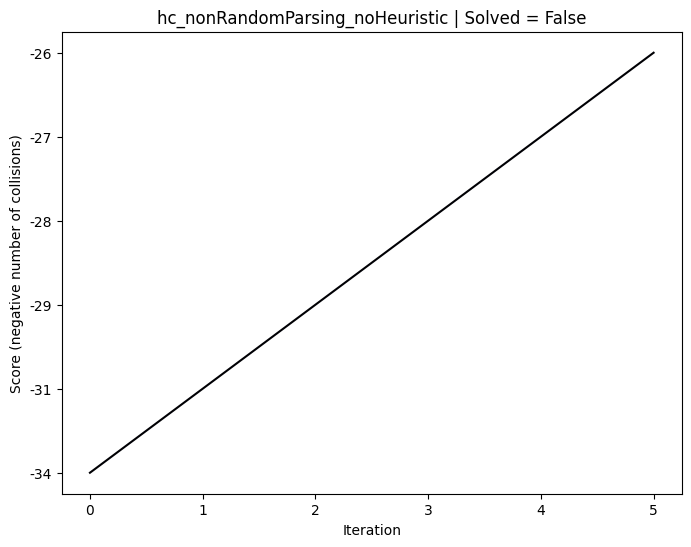
\includegraphics[width=0.34\textwidth]{plot_1.png}}
	\subfigure[]{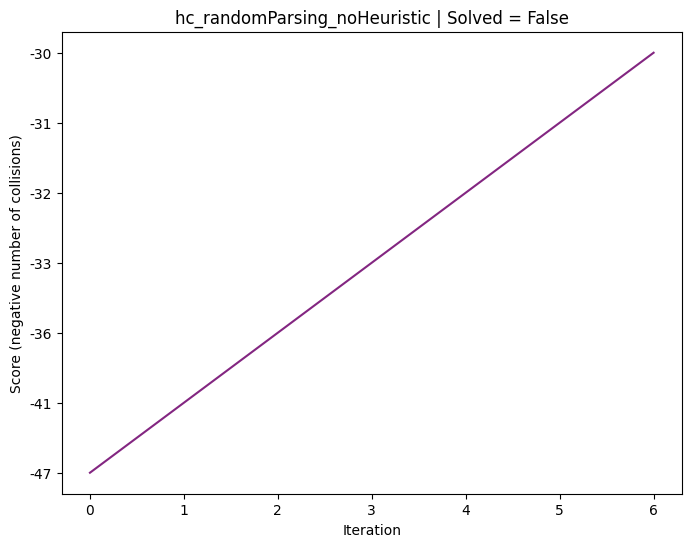
\includegraphics[width=0.34\textwidth]{plot_4.png}}
	\subfigure[]{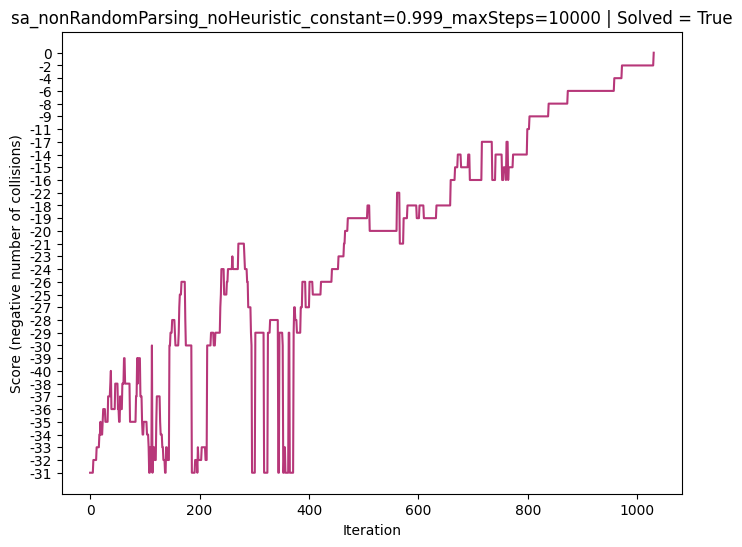
\includegraphics[width=0.34\textwidth]{plot_5.png}}
	\subfigure[]{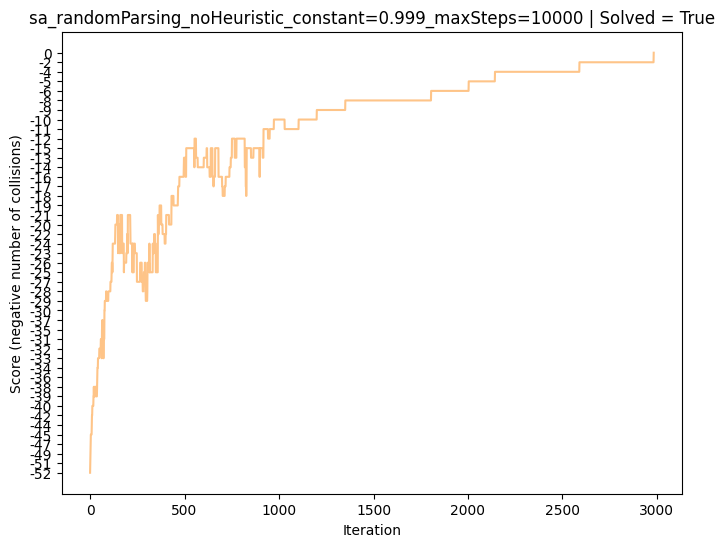
\includegraphics[width=0.34\textwidth]{plot_8.png}}
	\label{fig:foobar}
\end{figure}
\vspace{-20pt}

On voit de cette figure que le score, qui représente la valeur négative du
nombre de contradictions, a un comportement semblable
en général peu importe le parsing utilisés (non aléatoire à gauche et
aléatoire à droite). Il y a beaucoup plus de variations avec simulated
anealing comme il est attendu puisque l'algorithme peut choisir une solution
avec plus de contradictions selon la température. Sur l'axe du score, une valeur de
0 implique que le sudoku est résolu. On remarque alors que le hill climbing est
resté pris sur un maximum local et n'a pas réussit à résoudre le sudoku.

\section{Fonctionnement du code}
Le fichier à exécuter est sudoku.py. Il faut s'assurer que les fichiers
contenant des sudokus sont placés dans le même dossier que l'exécutable. Une
fois sudoku.py exécuté, les statistiques de résolution des sudokus seront
imprimées pour les différents algorithmes. Des fonctions utilitaires se trouvent
entre les lignes 50 et 69, les fonctions pour le DFS et les heuristiques entre
les lignes 69 et 214, les fonctions pour le hill climbing entre les lignes 214
et 388 et finalement les fonctions pour le simulated annealing entre les lignes
388 et 460. Les lignes 460 jusqu'à la fin sont dédiées aux fonctions utilitaires
et de tests. La signature de la fonction "solve\_all()" a été modifiée et ces
modifications sont expliquées dans la docstring.

% END OF DOCUMENT =====================================================================================================
% % List of figures/tables
% \pagebreak
% \begin{appendix}
%     \phantomsection\listoffigures
%     \phantomsection\listoftables
% \end{appendix}

\pagebreak\phantomsection\printbibliography[heading=bibintoc]
%\nocite{}
\end{document}
